%!TEX program = xelatex
\documentclass[10pt,english, openany]{book}
\usepackage{ctex, draftwatermark, everypage}

\SetWatermarkText{上海眼控科技股份有限公司}
\SetWatermarkLightness{0.95}
\SetWatermarkScale{0.4}


\usepackage[utf8]{inputenc} % allow utf-8 input
\usepackage[T1]{fontenc}    % use 8-bit T1 fonts
\usepackage{hyperref}       % hyperlinks
\hypersetup{colorlinks=true,linkcolor=black}
\usepackage{url}            % simple URL typesetting
\usepackage{booktabs}       % professional-quality tables
\usepackage{amsfonts}       % blackboard math symbols
\usepackage{nicefrac}       % compact symbols for 1/2, etc.
\usepackage{microtype}      % microtypography
\usepackage{pgfplots}
\usepackage{appendix}
\usepackage{longtable}
\usepackage{subfig}
\usepackage{graphicx}
\usepackage{animate}		% 动图

\usepackage{lipsum}
\setcounter{secnumdepth}{3}
\setcounter{tocdepth}{3}
\setlength{\parskip}{\smallskipamount}
\setlength{\parindent}{2pt}

\usepackage{verbatim}   % 注释

% Set page margins
\usepackage[top=100pt,bottom=100pt,left=68pt,right=66pt]{geometry}

% Changes the style of chapter headings
\usepackage{titlesec}
\titleformat{\chapter}
   {\normalfont\LARGE\bfseries}{\thechapter.}{1em}{}

\graphicspath{ {fig/} }

%%%%%%%%%%%%%%%%%%%%%%%%%%%%%% Starts the document
\begin{document}

\begin{titlepage}
	\clearpage\thispagestyle{empty}
	\centering
	\vspace{1cm}

	% Titles
	% Information about the University
	{\normalsize Shanghai Em-Data Technology Co.,Ltd. \par}
		\vspace{2cm}
	{\Huge \textbf{基于泰州多普勒雷达的AI临近预报——数据训练结果汇报}} \\
	%\vspace{1cm}
	%{\large \textbf{xxxxx} \par}
	\vspace{10cm}
    
    \centering 
\includegraphics[scale=0.5]{logo3.png}
    
    \vspace{0.5cm}
		
	% Set the date
	{\normalsize 2020年07月24日 \par}
	
	\pagebreak

\end{titlepage}

% Adds a table of contents
\tableofcontents{}

%%%%% Text body starts here!
\mainmatter

\chapter{数据概览}

\section{数据接收}

\begin{table}[!htbp]
    \centering
    \resizebox{\textwidth}{!}{
    \begin{tabular}{|c|c|c|c|c|}
		\hline
		雷达站点 & 地区 & 型号 & 时间范围 & 作用\/备注 \\
		\hline
		\hline
		Z9523 & 泰州 & SA & 20200610-20200617 & 测试模型在没见过的泰州的效果及问题(20200708收到第一批数据) \\
		\hline
		Z9523 & 泰州 & SA & 20200618-20200630 & 加入模型训练,数据量增加半个月后效果(20200716收到第二批数据) \\
		\hline
    \end{tabular}}
\end{table}

\section{雷达信息}

\begin{table}[!htbp]
    \centering
    \resizebox{\textwidth}{!}{
    \begin{tabular}{|c|c|}
		\hline
		属性 & 说明 \\
		\hline
		\hline
        站点编号 & Z9523 \\
        \hline
        类型 & SA \\
        \hline
        雷达经度(E) & 119.99389 \\
        \hline
        雷达纬度(N) & 32.556945 \\
		\hline
		雷达高度(m) & 57.3 \\
		\hline
		探测半径(KM) bins*Rreso & 460 x 1km=460 \\
		\hline
		时间分辨率(min) & 5-6 \\
		\hline
		仰角信息 & 0.48339844 1.36230469 2.28515625 3.29589844 4.21875 6.02050781 9.75585938 14.50195312 19.3359375 \\
		\hline
    \end{tabular}}
    \caption{泰州雷达基本信息}
\end{table}



\chapter{模型性能(非系统纯单模型效果)}

由于泰州并未上线我们的系统,所以下面展示的结果都是单纯AI模型的输出,没有加任何后处理和融合预报;

\begin{table}[h]\tiny
	\centering
	\resizebox{\textwidth}{!}{
	\begin{tabular}{|c|c|c|c|}
		\hline
		\multicolumn{3}{|c|}{测试集:江苏泰州雷达20200610-0617数据} & 训练集:江苏泰州雷达202006数据\\
		\multicolumn{3}{|c|}{数量:287, 测试员:MGD, 测试时间:20200709} & 测试集:江苏泰州雷达20200618-0630数据\\
		\hline
		指标 & 未训练泰州数据 & 加入泰州数据(batch1)训练 & 加入泰州数据(batch1+2)训练\\
		\hline
		AVG\_mse\_cloud\_ratio & 15.565851 & 10.21144 & 11.350837\\
		\hline
		AVG\_mse\_bigdbz\_cloud\_ratio & 20.790348 & 14.249949 & 15.492631\\
		\hline
		AVG\_psnr\_cloud\_ratio & 22.894097 & 28.060134 & 24.762837\\
		\hline
		AVG\_ssim\_cloud\_ratio & 0.771937 & 0.918532 & 0.838586\\
		\hline
		AVG\_corr\_cloud\_ratio & 0.789951 & 0.939649 & 0.88209\\
		\hline
		AVG\_csi\_10dbz\_cloud\_ratio & 0.515184 & 0.745195 & 0.5796 \\
		\hline
		AVG\_csi\_15dbz\_cloud\_ratio & 0.462389 & 0.675373 & 0.5181 \\
		\hline
		AVG\_csi\_20dbz\_cloud\_ratio & 0.397093 & 0.595826 & 0.4258 \\
		\hline
		AVG\_csi\_25dbz\_cloud\_ratio & 0.316317 & 0.529835 & 0.3254 \\
		\hline
		AVG\_csi\_30dbz\_cloud\_ratio & 0.209591 & 0.430391 & 0.2155 \\
		\hline
		AVG\_csi\_35dbz\_cloud\_ratio & 0.099419 & 0.286623 & 0.1012 \\
		\hline
	\end{tabular}}
	\caption{虹桥模型在泰州20200610-0617上的测试指标结果(最后一列为在泰州20200618-0630上测试)。可以看到加入了泰州数据进行训练后,指标普遍提升,模型可以很好的适应泰州数据。}
	\label{tab: ygnet_hongqiao4taizhou_test}
\end{table}

\section{模型泛化能力——虹桥模型在泰州的应用}

2020年7月7日我们收到江苏省台提供的8天的泰州雷达数据,我们将我们在上海上线的临近预报系统的AI模型进行直接外推,
由于不同地区本身的天气特点和对流的发展情况均有不同,所以这个模块我们主要看未接触泰州数据的虹桥模型在泰州数据上
的表现能力。这个模块也能看出我们的模型在非地域性性质的学习主要体现在哪方面。而模型在已经见过的泰州的天气过程的效果
见章节\ref{sec: model_learn}。

\textbf{学习数据:} 虹桥雷达数据 -> \textbf{推理(外推)数据:} 泰州雷达20200610-0617数据。

\subsection{个例分析}

\textbf{结论:}测试结果表明,模型能够捕捉到增长和消散趋势,但是也有部分数据存在消散过快的问题,可能是由于测试的数据与训练集差别过大导
图\ref{fig:sample4}是020年06月13日08:22:00泰州雷达的一个对流生成过程,第一行为输入的历史1h实况(10帧),第二行为未来2h的实况(20帧), 第三行为模型预测的未来2h(20帧)。
可以看到,我们的模型在对流生成的情况下发展形态和位置依然比较准确,且2h后的预报细节和强回波预测依然很稳定。但是中间有一部分的强回波的强度预测有些偏差。

我们的模型在对流运动及发展状态的学习能力上一直很强,在强回波的学习能力及点对点的准确性上还有提升空间。同时也可以看出来,学习后的状态比之前对于过程的持续时间的把控更加稳定。

致。

如图\ref{fig:sample1}所示,第一行为实况的20帧(未来2小时),第二行为对应时间我们模型外推结果。本次案例存在两个对流,右上角是一个消散过程,
而左下角是一个对流发展增强的过程,预测值从趋势上来看增长趋势和消散趋势都已经捕捉到。

但是由于从来没有见过泰州的数据,所以对于强回波(大于35dBz)的预测能力并不足,并且模型倾向于预测消散过程。如图
\ref{fig:sample2}所示,整个对流的发展区域及变化基本能够捕捉,但是模型消散的比较快。其中一个原因是因为虹桥
的数据一个对流的维持一般持续并不是很长时间,模型性能很大程度取决于学习的数据。但是对流的生消变化趋势及位置是模型
学到的通用性的能力。

\begin{figure}
	\centering
	\centering 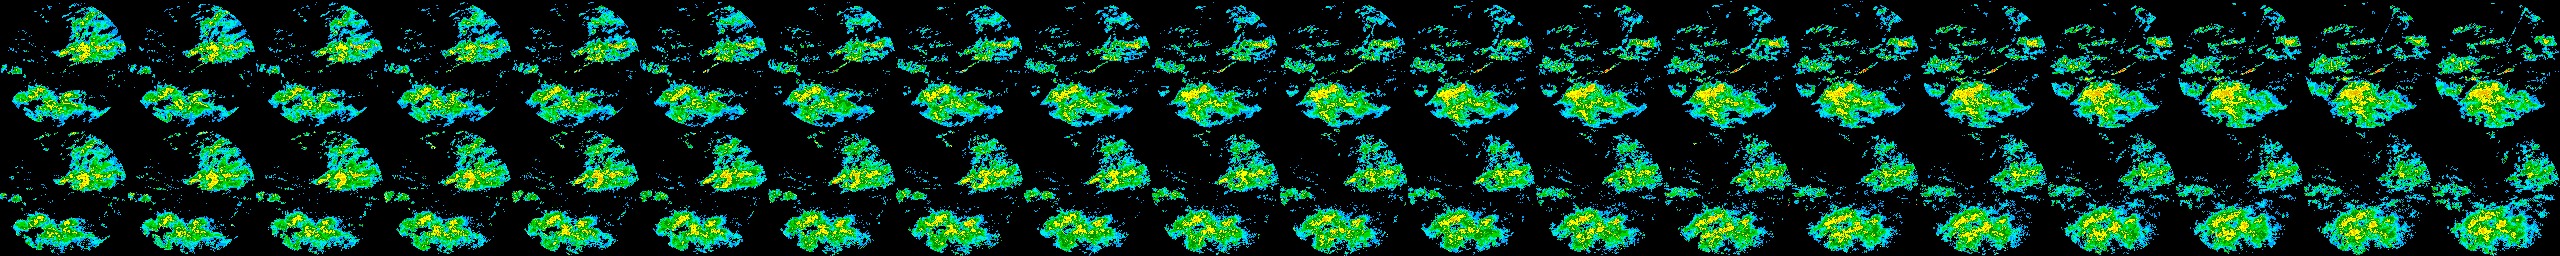
\includegraphics[scale=0.2]{sample1.png}
	\caption{第一行为实况的20帧(未来2小时),第二行为对应时间我们模型外推结果。预测值从趋势上来看增长趋势和消散趋势都已经捕捉到。}
	\label{fig:sample1}
\end{figure}

\begin{figure}
	\centering
	\centering 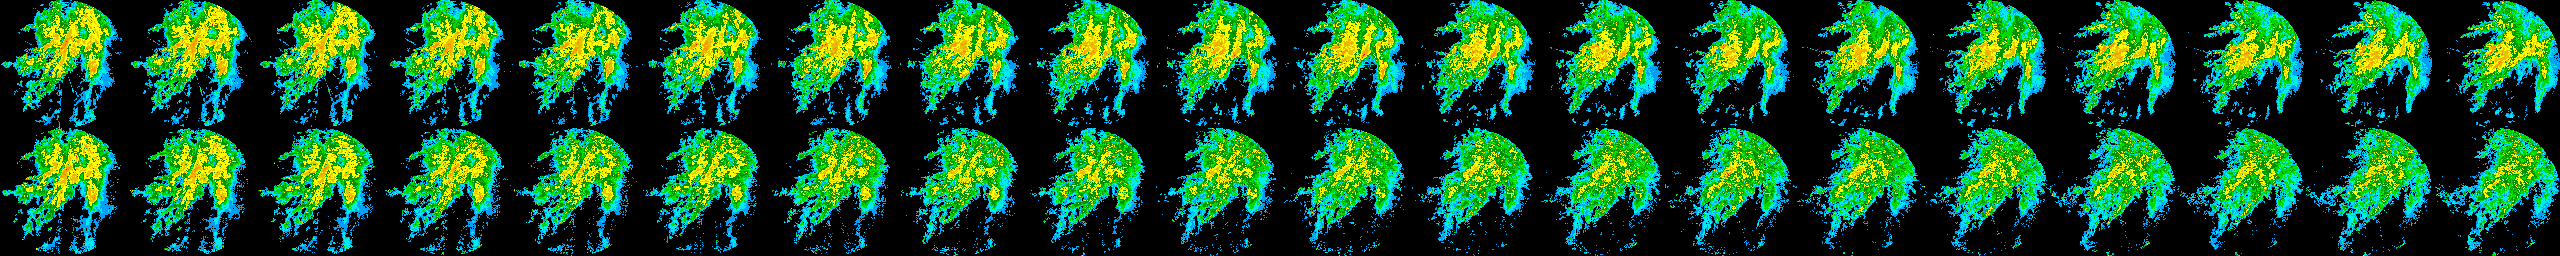
\includegraphics[scale=0.2]{sample2.png}
	\caption{第一行为实况的20帧(未来2小时),第二行为对应时间我们模型外推结果。模型消散的比较快。}
	\label{fig:sample2}
\end{figure}

\subsection{指标评估}

虹桥模型在泰州20200610-0617的数据(从未加入训练)上的整体测试效果如表\ref{tab: ygnet_hongqiao4taizhou_test}未训练泰州数据部分。对于没有训练过的数据,这个指标还是可以的。

指标都是每个案例都会不同,所以这里我们不要关心他的绝对值大小,由于指标大小本身和反射率因子占比有关,所以我们的指标根据不同的
反射率因子又有区分,具体每个指标代表的意思见章节\ref{chapter: index}。

\section{模型学习能力——泰州数据学习后在已学习泰州数据上的效果} \label{sec: model_learn}

我们将泰州雷达20200610-0617数据加入训练集,训练虹桥临近外推模型。测试结果表明我们的模型能够比较好拟合训练集。这个模块主要是看模型在泰州数据的学习能力的情况。

\textbf{学习数据:} 虹桥雷达数据+泰州雷达20200610-0617数据 -> \textbf{推理(外推)数据:} 泰州雷达20200610-0617数据。

\subsection{个例分析}

\textbf{结论:}测试结果表明我们的模型能够比较好拟合训练集。也就是说再学习过的天气过程会预测的非常好。

图\ref{fig:sample3}是2020年06月12日09:39:00泰州雷达的一个消散过程,第一行为输入的历史1h实况(10帧),第二行为未来2h的实况(20帧), 第三行为模型预测的未来2h(20帧)。
可以看到,我们的模型整体的发展形态和位置都比较准确,但是强回波的范围还是会偏小一些。动图效果如下(左侧为实况(红色边框),右侧为模型预测结果(绿色边框)。如果看得不是动图,需要换PDF阅读器或者见附件的单帧图片):

\begin{center}
	\animategraphics[width=18cm,height=9cm, autoplay, loop, controls]{2}{Z_RADR_I_Z9523_20200612093900_O_DOR_SA_CAP.png-}{0}{29}
	% \caption{2020年06月12日09:39:00 Z9523雷达组合反射率模型预测对比动图(消散过程)}
\end{center}

图\ref{fig:sample4}是2020年06月13日08:22:00泰州雷达的一个对流生成过程,第一行为输入的历史1h实况(10帧),第二行为未来2h的实况(20帧), 第三行为模型预测的未来2h(20帧)。
可以看到,我们的模型在对流生成的情况下发展形态和位置依然比较准确,且2h后的预报细节和强回波预测依然很稳定。但是中间有一部分的强回波的强度预测有些偏差。动图效果如下(左侧为实况(红色边框),右侧为模型预测结果(绿色边框)。如果看得不是动图,需要换PDF阅读器或者见附件的单帧图片):

\begin{center}
	\animategraphics[width=18cm,height=9cm, autoplay, loop, controls]{2}{Z_RADR_I_Z9523_20200613082200_O_DOR_SA_CAP.png-}{0}{29}
	% \caption{2020年06月13日08:22:00 Z9523雷达组合反射率模型预测对比动图(生成过程)}
\end{center}

我们的模型在对流运动及发展状态的学习能力上一直很强,在强回波的学习能力及点对点的准确性上还有提升空间。同时也可以看出来,学习后的状态比之前对于过程的持续时间的把控更加稳定。

\begin{figure}
	\centering
	\centering 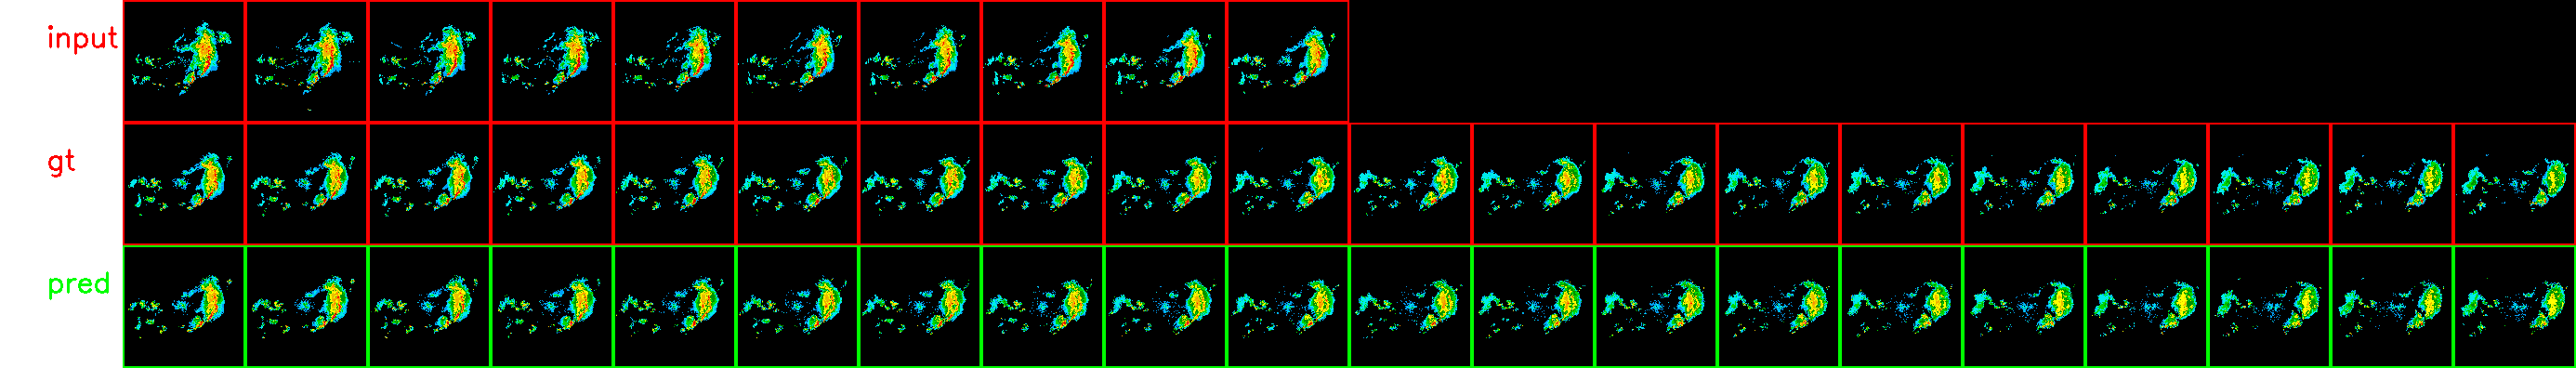
\includegraphics[scale=0.18]{Z_RADR_I_Z9523_20200612093900_O_DOR_SA_CAP.png}
	\caption{2020年06月12日09:39:00 Z9523雷达组合反射率模型预测对比图(消散过程)。第一行为输入的历史1h实况(10帧),第二行为未来2h的实况(20帧), 第三行为模型预测的未来2h(20帧)。可以看到我们的模型的消散过程学习的非常好}
	\label{fig:sample3}
\end{figure}

\begin{figure}
	\centering
	\centering 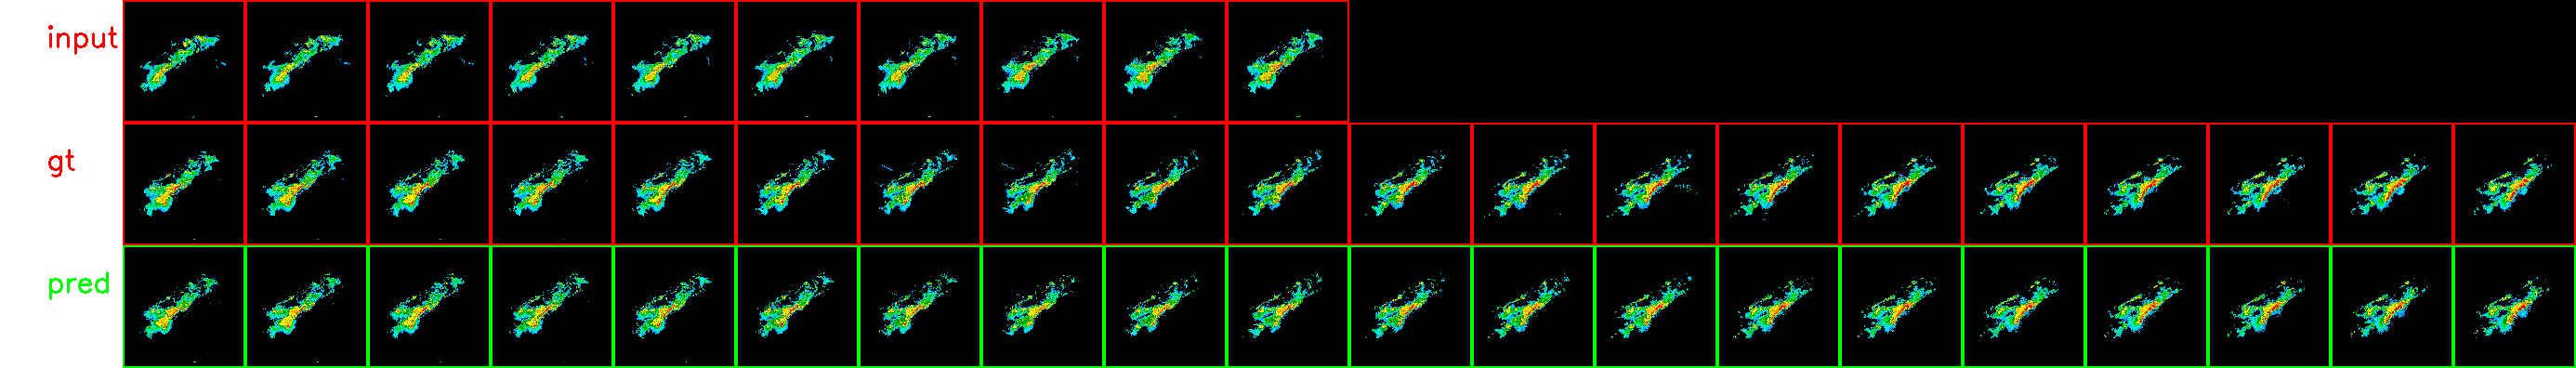
\includegraphics[scale=0.18]{Z_RADR_I_Z9523_20200613082200_O_DOR_SA_CAP.png}
	\caption{2020年06月13日08:22:00 Z9523雷达组合反射率模型预测对比图(生成过程)。第一行为输入的历史1h实况(10帧),第二行为未来2h的实况(20帧), 第三行为模型预测的未来2h(20帧)。可以看到我们的模型的部分强回波预测片弱,但整体生成趋势一致且2h后依然稳定。}
	\label{fig:sample4}
\end{figure}

\subsection{指标评估}

虹桥模型加入泰州20200610-0617的数据测试指标效果如表\ref{tab: ygnet_hongqiao4taizhou_test}加入泰州数据bath1部分。可以看到,加入数据训练后,指标全面提升,我们的模型
在已经学习过的天气过程中预报的很好。但是对于强回波的准确预报还有很大提升空间。下一部分我们分析有更多训练数据后,模型在泰州的表现效果。


\section{模型鲁棒能力——泰州数据学习后在未学习泰州数据上的效果}

2020年7月17日我们收到了省台提供的2020年06月18日至2020年6月30日的泰州雷达数据。我们将其加入训练,由于加入数据训练比较晚,所以模型还没有完全收敛,
目前结果已经形态上已经比较相似,强回波的移动也基本一致。

\textbf{学习数据:} 虹桥雷达数据+泰州雷达20200610-0630数据 -> \textbf{推理(外推)数据:} 泰州雷达20200618-0630数据。

\subsection{个例分析}

\textbf{结论:} 加入更多数据之后,模型具备一定的抗噪能力。目前还没有完全训练收敛,目前的结果已经形态上已经比较相似,强回波的移动也基本一致。
希望得到更多的数据加入训练,并且可以先上线AI临近外推系统,使用在线学习不断的对模型进行迭代优化。部署所需环境见章节\ref{chapter: build}。

图\ref{fig:sample5}是2020年06月19日10:21:00泰州雷达的一个过程,第一行为输入的历史1h实况(10帧),第二行为未来2h的实况(20帧), 第三行为模型预测的未来2h(20帧)。
实况中在第6帧(未来半小时后)和第11帧之后(未来一小时后)有些射线噪声,但是我们的模型预测的结果并不会预测噪声,所以有去噪的能力。
模型知道哪些是噪声哪些是蕴含外推信息量的特征点。

\begin{figure}
	\centering
	\centering 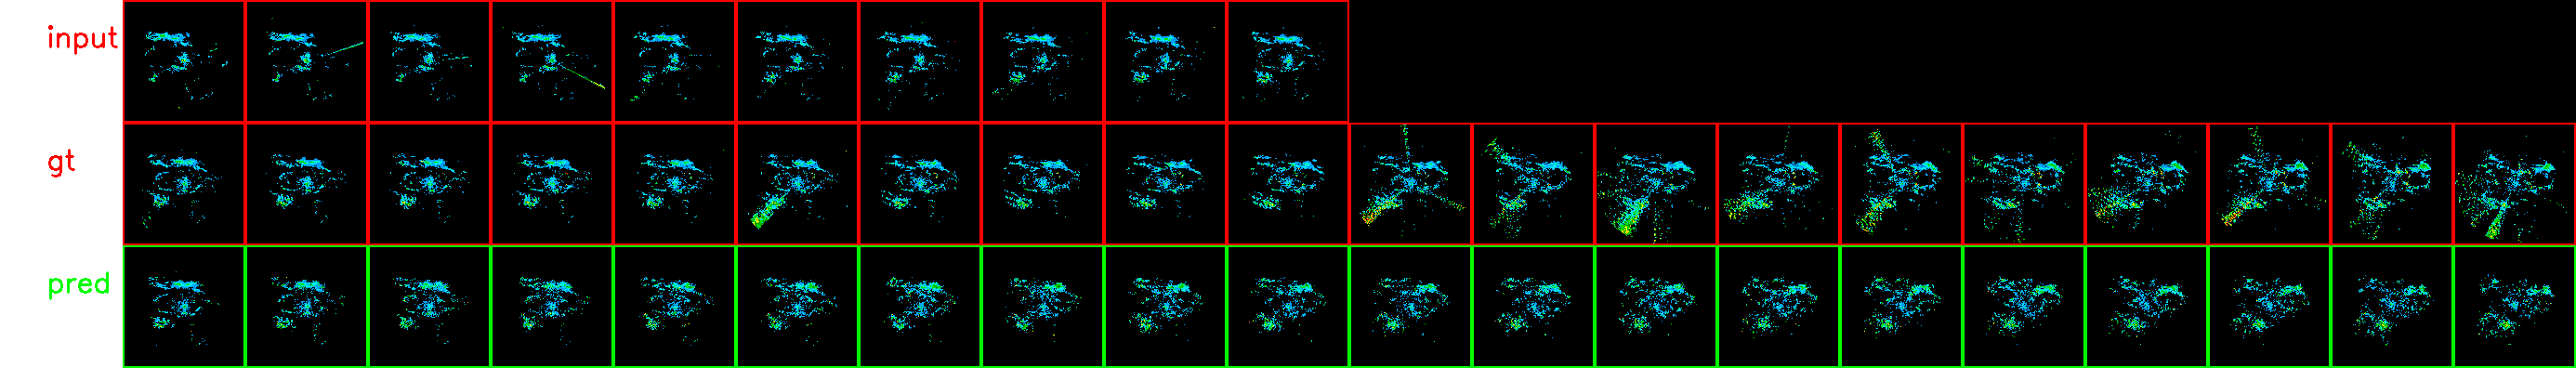
\includegraphics[scale=0.18]{Z_RADR_I_Z9523_20200619102100_O_DOR_SA_CAP.png}
	\caption{2020年06月19日10:21:00 Z9523雷达组合反射率模型预测对比图(模型抗噪)。第一行为输入的历史1h实况(10帧),第二行为未来2h的实况(20帧), 第三行为模型预测的未来2h(20帧)。可以看到我们的模型的在gt含噪声的时候依然可以形态预测的很好,并且自动过滤了噪声。}
	\label{fig:sample5}
\end{figure}

图\ref{fig:sample6}是2020年06月19日12:26:00泰州雷达的一个过程,第一行为输入的历史1h实况(10帧),第二行为未来2h的实况(20帧), 第三行为模型预测的未来2h(20帧)。
输入网络的每一帧都有一些射线噪声,但是我们的模型预测的结果并不会预测噪声,而且预测的状态也比较稳定。所以模型具备噪声抗干扰的能力。

\begin{figure}
	\centering
	\centering 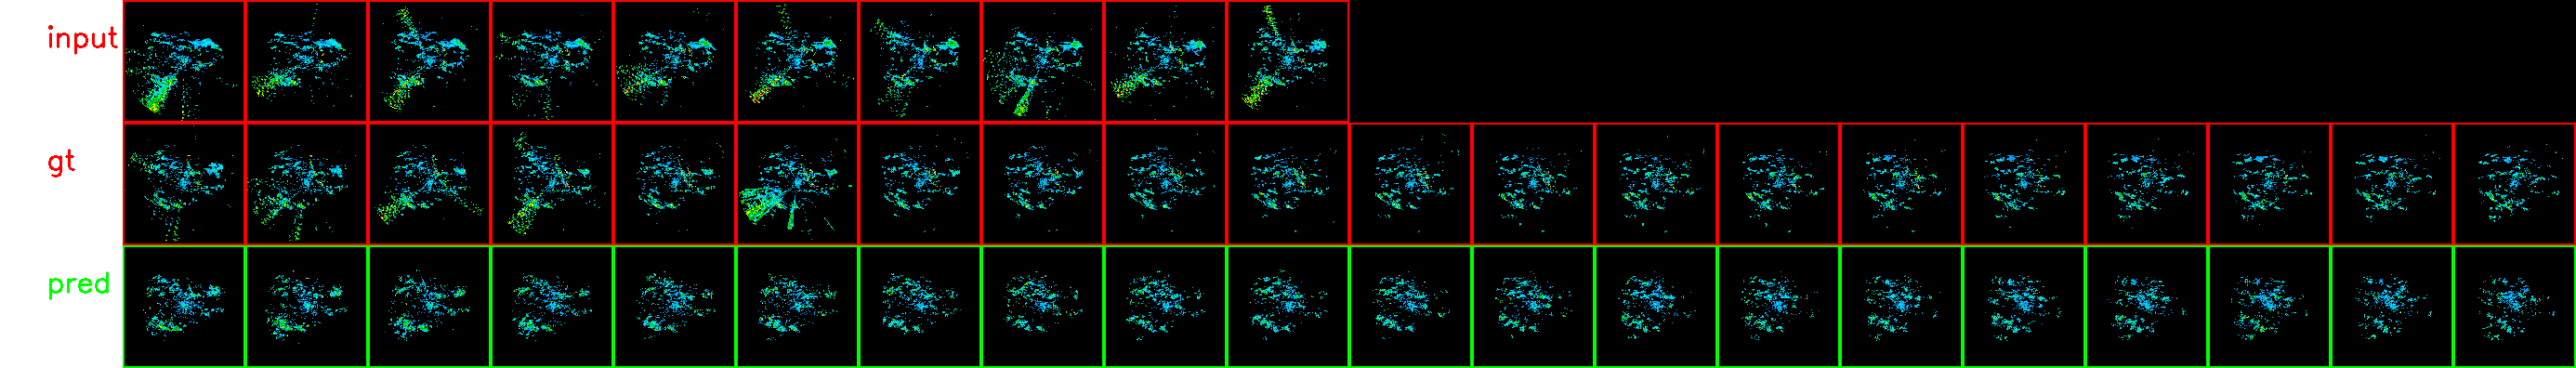
\includegraphics[scale=0.18]{Z_RADR_I_Z9523_20200619122600_O_DOR_SA_CAP.png}
	\caption{2020年06月19日12:26:00 Z9523雷达组合反射率模型预测对比图(模型抗噪)。第一行为输入的历史1h实况(10帧),第二行为未来2h的实况(20帧), 第三行为模型预测的未来2h(20帧)。可以看到我们的模型的在输入含噪声的时候依然可以形态预测的很好,并且自动过滤了噪声。}
	\label{fig:sample6}
\end{figure}

图\ref{fig:sample7}是2020年06月16日21:44:00泰州雷达的一个对流生成过程,第一行为输入的历史1h实况(10帧),第二行为未来2h的实况(20帧), 第三行为模型预测的未来2h(20帧)。
外推的效果整体形态及运动趋势均和实况一致,但是强回波的预测状态并不是很稳定,也有可能是模型还没有收敛,泰州半个月的数据过少相关。

\begin{figure}
	\centering
	\centering 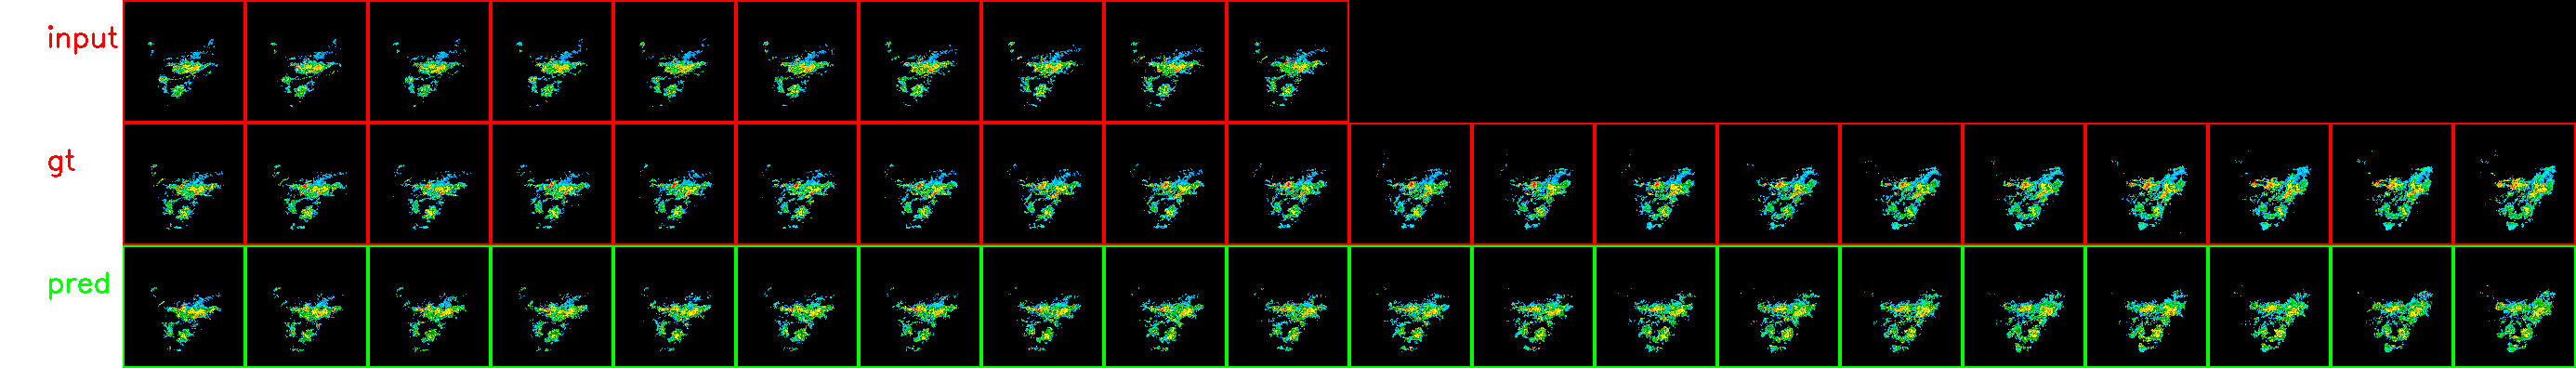
\includegraphics[scale=0.18]{Z_RADR_I_Z9523_20200626214400_O_DOR_SA_CAP.png}
	\caption{2020年06月26日21:44:00 Z9523雷达组合反射率模型预测对比图(强回波状态不稳定)。第一行为输入的历史1h实况(10帧),第二行为未来2h的实况(20帧), 第三行为模型预测的未来2h(20帧)。可以看到我们的模型对流运动和区域稳定,但是强回波的预测不稳定。(模型还没有收敛)}
	\label{fig:sample7}
\end{figure}

模型更多外推效果见附件压缩包"YGNet在泰州06月的表现效果.zip"。(左边为实况,右边为模型输出/外推。红色为实况或者输入,绿色为AI外推。)

\subsection{指标评估}

详细指标见表\ref{tab: ygnet_hongqiao4taizhou_test}。 对比最后三列可以看出模型正在不断的提升性能,还没有达到“加入泰州数据(batch1)训练”的效果,
但是已经比从未训练的好很多,说明模型还未收敛。但是整个形态上已经很不错了。

\chapter{指标评估} \label{chapter: index}

\begin{enumerate}
    \item SSIM(Structural Similarity Index)(值域为[0, 1], 越趋近1越好);
    
    作为结构相似性理论的实现,结构相似度指数从图像组成的角度将结构信息定义为独立于亮度、对比度的,反映场景中物体结构的属性,并将失真建模为亮度、对比度和结构三个不同因素的组合。用均值作为亮度的估计,标准差作为对比度的估计,协方差作为结构相似程度的度量。给定两个图像$x$和$y$, 
    $$ SSIM(x, y) = \frac{(2\mu_{x}\mu_{y})(2\sigma_{xy}+c_2)}{(\mu_{x}^2 + \mu_{y}^2 + c_1)(\sigma_{x}^2 + \sigma_{y}^2 + c_2)} $$ 其中$\mu_x$是$x$的平均数,$\mu_y$是$y$的平均数, $\sigma_x^2$是$x$的方差,$\sigma_y^2$是$y$的方差, $c_1 = (k_1L)^2$, $c_2 = (k_2L)^2$是用来维持稳定的常数,$L$是像素值的动态范围。我们取$k_1 = 0.01$, $k_2 = 0.03$.

    \item MSE(Mean squared error)(阈值[0, n],越趋近0越好,n与图像大小及像素范围相关);
    $$ MSE = \frac{1}{N} \sum_{i=1}^{N} (y_i - \hat{y}_i) $$ 其中$y_i$表示第$i$个像素点对应的真实强度值,$\hat{y}_i$表示第$i$个像素点对应的预测强度值。
    
    \item CSI(Critical Success Index)(值域为[0, 1], 越趋近1越好);
    
    CSI是一个离散的评价指标,比如CSI-30表示以30dBZ为阈值,大于30dBZ的为1, 小于为0, 计算公式如下 $$CSI = \frac{hits}{hits+misses+falsealarms}$$ 可以用于关注不同强度阈值情况下模型的性能。但是目前这个指标依然是点对点并没有时序性。我们是实际应用中,回波强度阈值的间隔为5dBZ。
    
    \item PSNR(Peak signal-to-noise ratio);
    
    $$PSNR = 10 log_{10}(\frac{MAX_I^2}{MSE})$$, 其中$MAX_I^2$为图片中可能的最大像素值。
    
    \item FID(Fréchet Inception Distance);
    
    FID是计算了真实图片和假图片在 feature 层面的距离。弱化了像素点间的差异,更看中序列/单帧图像具备的特征差异。这里的特征网路可以是普通的inceptionV3,也可以是上面我们优化的对流运动分析模块、历史帧信息评估模块或对流生命周期预测模块的特征提取层。$$ FID = || \mu_r - \mu_g ||^2 + T_r(\sum_r + \sum_g - 2(\sum_r \sum_g)^{1/2} )$$,其中$\mu_r$为真实图像的特征的均值,$\mu_g$为预测图像的特征的均值,$\sum_r$为真实图像的特征的协方差矩阵,$\sum_g$为预测图像的特征的协方差矩阵。
    

\end{enumerate}

\chapter{系统部署} \label{chapter: build}

考虑到不同情况下使用有不同的需求,如没有可以支撑深度学习跑推理/系统的服务器或者显卡资源等情况,我们支持本地化部署和线上远程部署服务两种模式。
    
本地化系统所需的环境配置见表\ref{tab6.2}, 远程服务所需要的数据及接口见表\ref{tab6.3}
\begin{table}[htbp]
\centering
\begin{tabular}{|c|l|}
	\hline
	系统 & Ubuntu 16.04\\
	\hline
	硬件推荐配置 & 8核cpu, 2.2G hz以上; 内存16G以上; 硬盘2TB以上; \\
	\hline
	显存推荐配置 & tesla v100/ GeForce RTX 2080; \\
	\hline
	软件需求 & jdk 1.8,MySQL 5.7,ActivateMQ 5.15, Redis 4.0.8, nginx 1.10.3; python3;\\
	\hline
	框架需求 & tensorflow 1.15, pytorch 1.4  CUDA10 cuDNN7.5;\\
	\hline
\end{tabular}
\caption{本地化部署配置}
\label{tab6.2}
\end{table}

\begin{table}[!htbp]
\centering
	\begin{tabular}{|c|l|}
	\hline
	数据 & 雷达原始文件实时数据 \\
	\hline
	方式1 & ftp接口,雷达文件由对方推送到指定的ftp目录中\\
	\hline
	方式2 & http接口,提供获取最新雷达文件的http接口 \\
	\hline
	\end{tabular}
\caption{远程服务所需要的数据及接口}
\label{tab6.3}
\end{table}



\end{document}
